\documentclass[conference]{IEEEtran}

\IEEEoverridecommandlockouts
% The preceding line is only needed to identify funding in the first footnote. If that is unneeded, please comment it out.
\usepackage{cite}
\usepackage{amsmath,amssymb,amsfonts}
\usepackage{algorithmic}
\usepackage{graphicx}
\usepackage{textcomp}
\usepackage{xcolor}
\usepackage{listings}
\graphicspath{{./images/}}
\def\BibTeX{{\rm B\kern-.05em{\sc i\kern-.025em b}\kern-.08em
    T\kern-.1667em\lower.7ex\hbox{E}\kern-.125emX}}
\begin{document}

\title{A Fully Decentralized Infrastructure for Automated and Trusted IoT Data Trading}
% Chinese title: 針對物聯網資料交易的去中心化基礎建設

\author{\IEEEauthorblockN{1\textsuperscript{st} Ching-Hua (Vivian) Lin}
\IEEEauthorblockA{\textit{dept. of CSIE} \\
\textit{National Cheng Kung University}\\
Tainan City, Taiwan (R.O.C.) \\
jkrvivian@gmail.com}
\and
\IEEEauthorblockN{2\textsuperscript{nd} Ching-Chun (Jim) Huang}
\IEEEauthorblockA{\textit{dept. of CSIE} \\
\textit{National Cheng Kung University}\\
Tainan City, Taiwan (R.O.C.) \\
jserv@ccns.ncku.edu.tw}
\and
\IEEEauthorblockN{3\textsuperscript{rd} Chia-Heng Tu}
\IEEEauthorblockA{\textit{dept. of CSIE} \\
\textit{National Cheng Kung University}\\
Tainan City, Taiwan (R.O.C.) \\
chiaheng@gmail.com}
}

\maketitle


\begin{abstract} 
The Internet of Things (IoT) makes our lives simple and easier by automating mundane processes with devices around us. Within IoT scenarios, machine-to-machine (M2M) is an inevitable technology that allows machines to own their digital assets and start participating in an economy with other machines, which devices can share and trade their resources. For instance, smart meter data can assist in energy transition. Meanwhile, time smart meter data is privacy-sensitive, that implies power consumption can be associated with appliances used and eventually can be used to track somebody's behavior and location. Questions such as data ownership, data integrity and data privacy become new challenges in M2M economy. In this paper, we leverage usages of distributed ledger techonologies (DLTs) to construct an IoT-enabled, decentralized and trusted data marketplace on top of the IoT brokered infrastructure, in order to address the technical challenges. This approach can efficiently enhance the degree of transparency and scalability. The storage via an end-to-end encrypted message streams allows transmitting, accessing and validating data streams over distributed ledgers. Finally, we implement and evaluate the performance of the prototype.
\end{abstract}

\begin{IEEEkeywords}
Data Marketeplace, decentralization, Distributed Ledger Technology
\end{IEEEkeywords}

\section{Introduction}
%TODO: cite examples
In IoT, the development of M2M technology\cite{M2M}, cyber physical system (CPS)\cite{CPS} ,and Industry 4.0 grow rapidly. As the physical and digital data are deeply intertwined, the interactions among digital twins act as data exchanges\cite{digitaltwin} which brings potential value to IoT applications, such as health care\cite{healthCare}, factories ,and vehicles\cite{AutonomousDriving}, and brings up new business models where data is considered as tradeable digital assets. With the diverse data streams generated by different entities and carried across organizations among expanding the amount of interconnected devices, it is a challenge for data holders to share and track their data assets. Therefore, data marketplace is viewed as a solution to build a secure, reliable and scalable data sharing platform where data providers ,and data consumers meet.

Among the challenges of data marketplace\cite{BigDataMarket}, we conclude the following four essential requirements of a data marketplace system:
\begin{itemize}
	\item \textbf{Scalability}. 
1) The performance of data marketplace should scale with the massive amount of participants. 2) The keys and entry points of data products managed by participants should be as small as possible. 
	\item \textbf{Integrity}. 1) Prevent unauthorized modifications. 2) Ensure the accuracy and validity of contents.	
	\item \textbf{Confidentiality}. 
1) Only the authorized participants can access data streams. 2) Participants that have access can always retrieve data even if they're dropped from the network.	
	\item \textbf{Privacy}. Avoid revealing sensitive information of all participants, such as IP address and data consumers' habits which may leak within the subscription history.
	\item \textbf{Economics Incentive}. The economic incentives can encourage the data providers to participate in the system and pay more attention to the quality control. 
\end{itemize}

In contrast to centralized architectures in \cite{DIaas, IOTAIdustryMarketplace, MARSA} that target to handle static data sets, we proposed a decentralized data marketplace in \cite{MyDataMarketplace} which focuses on processing the high volume, high velocity and high variety of "Big Data" streams\cite{BigData} while fulfills the aforementioned requirements. Moreover, a decentralized architecture can better adapt the dynamic roles than a centralized one. See Fig.~\ref{fig:system_design}.

In the previous paper, we investigated the use of decentralized publish/subscribe (pub/sub) model and DLTs to construct the authority-less and trusted infrastructure, particularly Ethereum Smart Contract\cite{smartContract} and IOTA Masked Authenticated Messaging (MAM)\cite{MAM}. The pub/sub model features the scalability and resource-efficiency, and the economic incentives are stimulated by regulating trading agreement and penalty on Ethereum Smart Contracts with transparency. Lastly, MAM as the data storage not only ensures the data integrity, but also enables access control and provides a scalable key and data management. These three keys meet the requirements mentioned previously.   


\subsection{Contributions}
The contributions in the paper are summarized as follow:
\begin{itemize}
	\item Standing on our proposed decentralized data marketplace, we review several decentralized data marketplace architectures as well as the existing distributed storage, and clarify the necessity of using MAM.  
    \item We make an in-depth analysis of each layer of MAM, in addition to the performance evaluation and optimization of the current implementation. We also compare the perfomance of exchanging different cryptosystems.
	\item We analyze the security concerns when offloading MAM operations to brokers, and propose a solution to resolve them.
\end{itemize}


\subsection{Paper Organization}
The rest of this paper is organized as follows. In Section~\ref{section:background}, the architecture of our proposed decentralized data marketplace is illustrated. In Section~\ref{section:relatedWork}, some related work of decentralized data marketplace, distributed data storage and use cases of MAM are analyzed. In Section ARCHI, the interactions of MAM and Ethereum Smart Contract in trading model is well explained. The analysis and improvement of MAM are given in Section MAM-EXP. In Section OFFLOAD, the security issues and methods of offloading MAM operations to brokers will be discussed carefully. Finally, we conclude the paper in Section CONCLUSION.


\begin{figure}[!t]
    \centering
    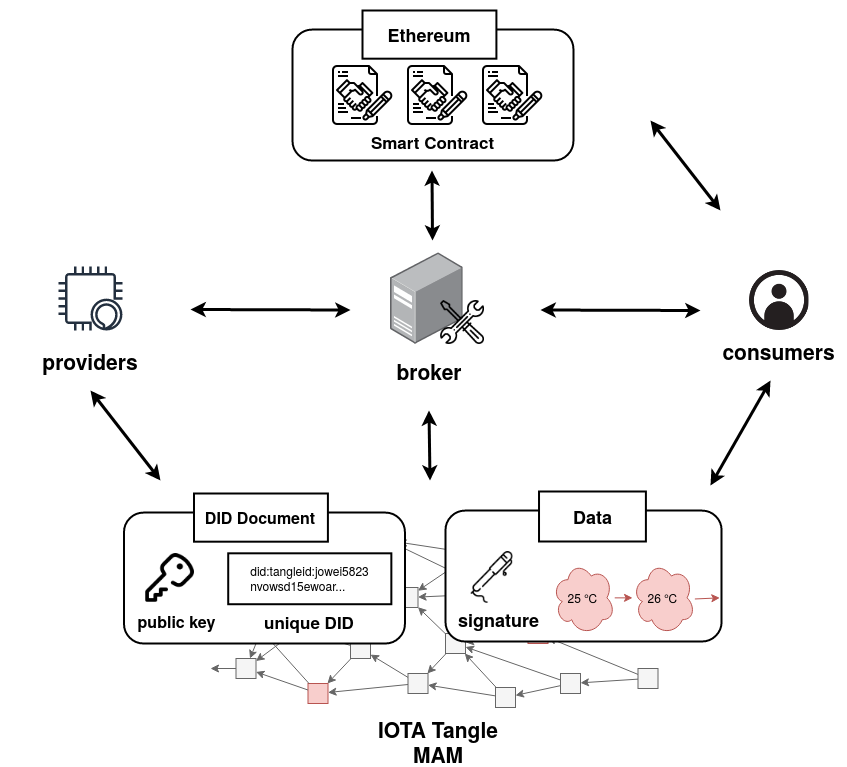
\includegraphics[width=3.in]{system_design}
    \caption{The system design of a decentralized data marketplace which consists of data providers, consumers and brokers.}
    \label{fig:system_design}
\end{figure}

\section{Related Work}
\label{section:relatedWork}
% pub/sub
\subsection{Data exchangement mechanism for IoT}
The publish/subscribe service model consists of publishers, subscribers and brokers, which has been proven\cite{pubSubAnalysis, pubSubAnalysis2} to be an efficient and flexible solution for a large number of diverse entities like IoT applications. A lot of work in publish/subscribe system focused on the scalability and the different security issues such as, encrypted data communication, privacy preserving data subscription and access control of digital asset. A few work targets on the storage which is a vital considerations for IoT and mobile computing and the incentive for data economics.

M. B. Abdullahi and G. Wang\cite{centralPubSub} presented a secure publish/subscribe data storage service in Wireless sensor networks (WSNs) which ensures several security issues. Each user has an identity for authentication, whereas subscribers' interests are encoded before matching to protect users' interests. Additionally, the proposed encryption scheme can prevent adversary to access published data if the sensor node is compromised. However, the access control and encryption keys of data is enforced by the network controllers (NCs) and Cirtificate Authorities (CAs), which may be a potential security risk of the system. Also the storage is not well illustrated in the work. G. S. Ramachandran et al.\cite{trinity} pointed out the security risk of centralized brokers, and applied DLTs to build a distributed pub/sub system which promotes the transparency of interactions of participants and the status of data. With the help of Smart Contract, usesrs can perform data validation easily, and brokers can keep track of data status. But data is plaintext on blockchain, which the privacy problem of sensitive data need to be considered carefully. The economics incentives that can encourage the publishers to participate the system and pay more attention on the quality control are not included. 

In \cite{userCentricData}, the publisher runs a node in blockchain that preserves all the history data of the ledger, therefore, they can publish and manage data without any third-parties. The subscribers request publisher directly and ask them to save a cache space for interested data. The main contribution of the system is to ensure data owners have full controls of produced data, but the data owners need to have well devices and environment to perform such functionalities and preserve data. Also, the rights for accessing digital assets is more compatible in the IoT scenarios instead of copying raw data. Secure Pub-Sub model\cite{SPS}, a brokerless of publish/subscribe model, is proposed to eliminate the security risk of middlewares in the model and to provide a reputation-based fairness payment strategy on blockcahin. The privacy and data security are considered thoroughly with the encryption scheme, while the reputation of publishers, payment and data sharing are deployed on smart contracts that allows all operations are transparent. The reputation system and the punishment rules against malicous acts of subscribers and publishers. Yet, without brokers, providers and subscribers may need to reveal more sensitive information like IP address in order to match the both sides. Another broker-less model in \cite{PrivacyPreservPubSub} protects the subscribers' privacy by encrypting users' interests with the light-weight PKEwET\cite{PKEwET}, which allows publishers to match the subscribers' interests in cipher text. 

\subsection{Decentralized Data Marketplace Infrastructure}
% decentralized DM

\subsection{Distributed Storage System}
% distributed data storage
Decentralized storage systems allow users to store files in a distributed network that is maintained by individual nodes around the world instead of a central service provider. Nevertheless, DLTs are often used as the backbone of these systems as data storage and also an incentive layer to encourage people get involved in the network. Filecoin \cite{FileCoin} in Inter-Planetary File system(IPFS)\cite{IPFS} is an incentive layer to incent nodes to provide storage. IPFS is a content-based addressing storage model in a peer-to-peer network, which users can obtain the data with the unique hash value through the network. However, no cryptographic system is applied for user-uploaded files. Sia\cite{Sia} splits the uploaded file into multiple data segments encrypted with the owner's private key, then cipher text is sent to the Sia nodes that rent the storage in Siacoin through smart contracts. Files are duplicated in multiple nodes to prevent data loss.

 
\section{System Design Thinking}
\subsection{The Architecture}
% TODO: pub/sub model selection
There are three major roles, data providers, data consumers and brokers in the decentralized data marketplace which is similar to the pub/sub messaging model. But unlike the standard pub/sub model where brokers link the publishers and subscribers who are not aware of each others. In our proposed architecture, the brokers are only responsible for message delivery and essential verification processes. Fig.~\ref{fig:system_design}

\begin{itemize}
\item \textbf{Data Provider: }
Data providers are the ones that generate streaming data and set the data price based on the different types of data. With the subscription fee that earned via trading, data providers are incentivized to maintain and improve the quality of data.
\item \textbf{Data Consumer: }
Data consumers are entities that are willing to buy data streams. As it is laborious to widely deploy devices to collect data from scratch, and without a marketplace, it is also difficult to find providers of the data sets, purchases is the fastet and efficient way to get the desired data sets. 
\item \textbf{Broker: }
Brokers are responsible for building an agreement between data providers and consumers. Also brokers can represent data providers to perform computing tasks as brokers are expected to have higher resource. 
\end{itemize}

% use IPFS as searching indexes
\subsection{Choice of Data Storage}
Data storage is an important element of data marketplace where the data assets are reserved. We assume such storage system should be distributed which runs on the peer-to-peer network maintiaining by multiple nodes. Hence, the risk of system paralysis for server being compromised or shutdown unexpectedly can be removed. Among the existing distributed storage mentioned in Section~\ref{section:relatedWork}, different architectures, back-up mechanisms and access controls strategies are proposed. Yet the keys and addresses of data managed by participants are hard to be as small as possible especially for data streams.  

% MAM
MAM publishes authenticated streaming data as zero-value transactions to IOTA ledger and provides the ability to publish and fetch encrypted messages over the IOTA Tangle along with data integrity and access control. With MAM, the rights of data access are traded instead of a copy of data in the data marketplace, which eliminates the need for data consumers to have additional storage.
 
In the IOTA protocol, \textbf{seed} is the identifier of its owner. An IOTA seed represents the ownership of all things associated with the user in the IOTA ecosystem, such as IOTA tokens or messages on the Tangle. With the seed, the owner can create addresses and signatures in order to issue transactions or publish messages to MAM channels and endpoints.

Either channel or endpoint is like a singly-linked list. The singly-linked list structure implements the concept of forward secrecy, where no one has access to the data back from his/her entry point. Furthermore, each address of a message can be derived from the previous one, which enables data consumers to subscribe to future data by having the endpoint ID. A MAM channel/endpoint ID is the address of a transaction and the first message of a channel/endpoint. The central endpoint in Fig.~\ref{fig:mam_struct} means its endpoint ID is the same as channel ID. 

A user can create multiple channels and endpoints, and the messages can be encrypted with the session key then broadcasted in chronological order to the Tangle by attaching it to an endpoint. This allows only authorized entities are able to decode these messages after retrieving them from the Tangle. 

\begin{figure}[!t]
    \centering
    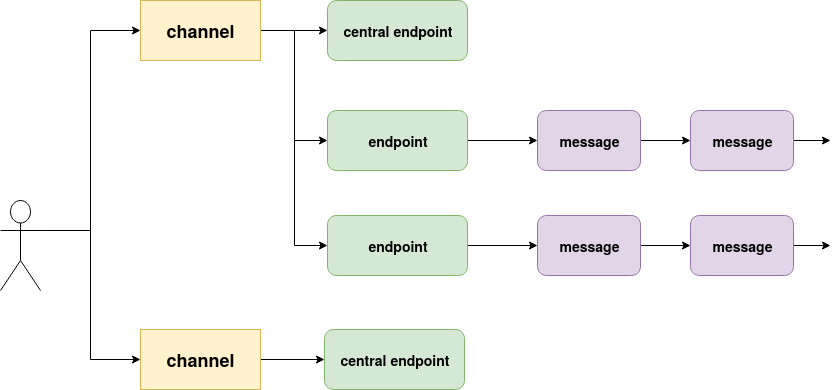
\includegraphics[width=2.5in]{mam_struct}
    \caption{The concept of MAM.}
    \label{fig:mam_struct}
\end{figure}

The authentication in MAM includes two aspects: source and data. Source authentication ensures the message that originates from the claimed owner, and data authentication ensures the integrity of the data from that sender. These are achieved through the Merkle signature scheme\cite{MSS} (MSS) which is a digital signature scheme based on Merkle Hash Trees and One-way hash functions. However, the size of Merkle Hash Trees, that is, the size of a channel/endpoint should be determined at the start. Thus, data providers need to first decide how to distribute data products into MAM channels/endpoints before uploading data.

Using MAM as a data storage benefits from the scalability of the underlying IOTA network as well as the decentralized and fault-tolerant characteristic of distributed ledgers, which reduce the risks of centralized storage services. 

%scalability
In our proposed architecture, MAM is the data storage which is the second layer data communication protocol built on top of IOTA\cite{IOTAwhitepaper} network, the Tangle, a feeless cryptocurrency designed for IoT. MAM allows users to put encrypted data streams into \textbf{channel}s and \textbf{endpoint}s, which consist of zero-value transactions on the Tangle. With an entry point (i.e., the address of transaction) and the encryption key, one can derive the following addresses of transaction and retrieve data. Table.~\ref{tab:mam_scalability} compares the key and addresses that need to be managed by using MAM and other distributed storage systems. Assuming the length of data stream is 7, and each record is encrypted with the same key. With MAM, only 1 key and 1 entry point is required while other distributed storage need to reserve 7 entry points for each data record.

\begin{table}[htbp]
	\caption{Number of keys and entry points of a data stream that need to managed with length 7.}
	\label{tab:mam_scalability}
	\begin{center}
	\begin{tabular}{|c|c|c|}
	\hline
		\textbf{Items} & \textbf{MAM} & \textbf{Others} \\ 
		\hline
		keys & 1 & 1 \\ 
		\hline
		entry points & 1 & 7 \\ 
		\hline
	\end{tabular}
	\end{center}
\end{table}

%classify
With the channel and endpoint structures, users can easily categorized data streams with respect to different types and usages. For instance, a voice assistant can create a channel every day with multiple endpoints for each gadgets to record daily logs. Another example is sensor devices like AirBox\cite{LASS}, collects environmental data, can split the statitics like PM 2.5 and humidity by time period into separate channels, which is useful for data providers to organize records and to pack into different data products. To do the classification in other distributed storage also encounters the aforementioned scalability problem, data entrypoints of the data steams should be reserved.    

%data trace
Moreover, data tracability is an important security issue that allows users to track the changes of data. Currently, hash is widely used to generate checksums of entire package of files, users can compare the hash value of files in order to check the integrity. Yet the hash values of each new version are unrelated and it's hard to point out the differences between versions. MAM benefits from the singly linked-list data structure which attaches messages chronologically, users can easily track the footprints of data change logs as well as checking the validity of modifications with the signature.

The operations of MAM are frequent, especially for data providers, who either upload data in a short time interval or maintain multiple MAM channels or endpoints at the same time, hence the operation of MAM is one of the potential bottleneck in data marketplace. In this paper, we evaluate the performance of MAM, and improve the effeciency with different strategies. Also, we take offloading the computation tasks to brokers as another possiblie approach for IoT devices, since brokers are considered to have higher computating power.

% alternative solution => IPFS(data) + MAM(index)

\subsection{Enable Automated Trading Process}
% Ethereum Smart Contract
% use ethereum smart contract => IOTA smart contracts are still under development
Ethereum is a cryptocurrency building on top of a public blockchain-based distributed ledger. 
It provides the smart contract, which is a protocol for formulating agreement on a blockchain that running on decentralized virtual machines. A smart contract can interact with other contracts, make decisions, store data and transfer cryptocurrency. All the participants in Ethereum can verify and execute the contracts, and once the contract is triggered, it will be executed automatically without any third-parties and it is uninterruptible. 

With the functionalities of Ethereum smart contracts, a flexible and verifiable trading mechanism can be acheived. \textbf{Product Contract} is made for the product launching and trading process in the decentralized data marketplace. The information of data products such as MAM channel ID (the data entry point), data price, time period and the broker-verified encryption key are listed on Product Contract. Furthermore, the participants can exchange encryption keys without any authorities via smart contracts. Though this design may cost extra transaction fees than exchanging key off-chain, it is considered a more secure strategy to protect the privacy of both providers and subscribers.



\section{Decentralized Data Marketplace Case Study}
Trading Models of Decentralized Data Marketplace
\subsubsection{Set Up}
All participants need to register on TangleID\cite{TangleID}, a self-soverign identity system built on top of MAM, enables authentication without any third party via a decentralized identifiers and a public/private key pair for authentication. 

\subsubsection{Launch Data Products}
To launch a data product, data providers need to create a MAM channel/endpoint and a Product Contract. However, considering IoT devices have no ability to handle both uploading data to MAM and interacting Ethereum smart contracts while collecting continuous data with low computing power, these works are offloaded to brokers. 

The details of data product, such as data price, MAM channel/endpoint ID and time period are listed on the Product Contract. As regard to the encryption key of data product, it is certified by a broker with blind signature\cite{blindSig}, a mechanism that allows users to sign contents without knowing it, and written the signed key on the Product Contract. This provides an approach for data consumers to verify the encryption key that avoid data providers frauding data consumers with a wrong one. The workflow is shown in Fig.~\ref{fig:launching_product}. 

Data providers start uploading data once the MAM channel/endpoint are created, each MAM message contains encrypted contexts along with signatures which allows data consumers to check the integrity. In addition, one can perform the signature validation without the encryption key on MAM.
 
\begin{figure}[!t]
    \centering
    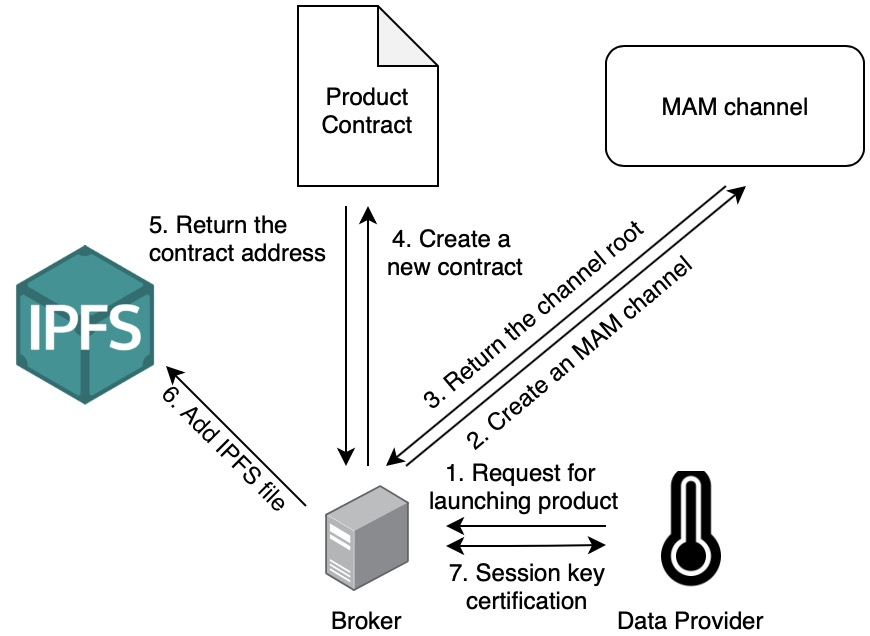
\includegraphics[width=2.5in]{launching_product}
    \caption{The process of launching a product.}
    \label{fig:launching_product}
\end{figure}

\subsubsection{Trading}
Data consumers pay subscription fees to the Product Contract of desired data products, and data providers give the "access" of data products on MAM instead of the files to consumers. The MAM channel/endpoint encryption key is encrypted with the public key of data consumer by data provider and written on the Product Contract, which ensures only data consumers can retreive it from Product Contract. 

Transferring the encryption key on smart contract instead of off-chain not only ensures the consistency of the encryption key but also prevents frauds from malicious participants. Furthermore, with the help of brokers and smart contracts, both data providers and consumers do not need to be online at the same time to proceed the trading process. The key sending process is shown in Fig.~\ref{fig:key_exchange}. 

\begin{figure}[!t]
    \centering
    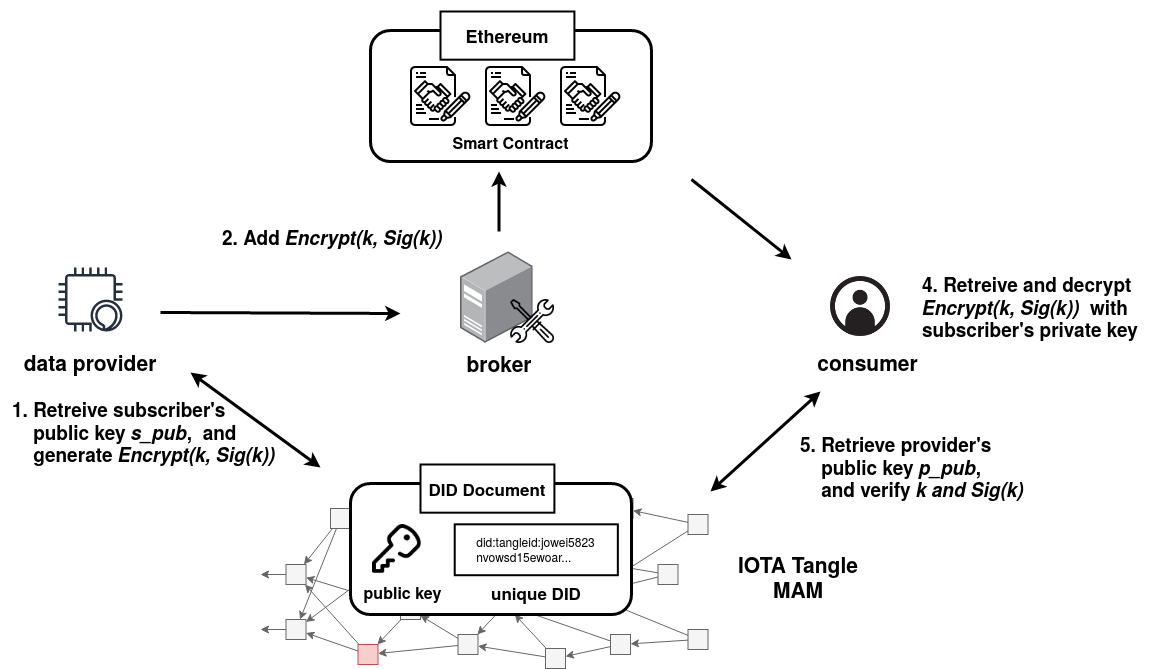
\includegraphics[width=3.5in]{key_exchange}
    \caption{Encryption key exchangement process.}
    \label{fig:key_exchange}
\end{figure}

\subsubsection{Refunding}
Subscribing to future data is a high-risk which data provider may not upload data as the agreement set after recieving the subscription fee. Therefore, in our proposed architecture, data consumers can initiate a refund procedure if the data is not available or defective. The subscription fee is transferred from the Product Contract to data providers when the committed data is available on MAM. When the refund procedure is launched, all consumers start voting based on their opinions on the data product. Once the ratio of consent votes of refunding is higher than a threshold, the subscription fee is proportionally transferred to the data provider, broker and every consumer. 


\section{Evaluations}
It is worth making a claim that all participants in data marketplace do not need to hold an IOTA full node which maintains the transaction history and exchanges information of the Tangle. Each role is only required to run client libraries and communicate with IOTA full nodes to interact with the Tangle. Therefore, in the following evaluations, all devices run with client library only.

\subsection{MAM Performance Evaluation}
MAM is a secure and validatable data storage of the proposed architecture. And publishing data to MAM is the primary key to resolve all the difficulties discussed in previous sections. The interactions between data providers and MAM can be frequent. Data providers can either upload data in a short time interval or maintain multiple MAM channels or endpoints at the same time, hence the operation of MAM is one of the potential bottleneck in data marketplace.

In this section, time measurement is evaluated in two MAM operations: channel/endpoint creation and data attachment to endpoints. To perform the evaluation assessment, a personal computer (PC, 3.2GHz 64-bit 6-core i7-8700 with 16GB DDR4 RAM) and a Raspberry Pi 3 Model B (1.2 GHz 64-bit quad-core ARM Cortex-A53 with 1GB LPDDR2 RAM) have been used to run MAM. 

\subsubsection{Channel / Endpoint Creation}
The length of a channel or endpoint is $2^{height}-1$ where \textit{height} is the height of Merkle Hash Tree in a Merkle signature scheme (MSS), and the "$-1$" is for announcing the ID of next channel or endpoint. A channel with height $n$ can create $2^n-1$ endpoints, and an endpoint with height $m$ can attach $2^m-1$ messages, therefore the capacity of a channel is $2^{nm}-2^n-2^m+1$ messages in total. The greater the \textit{height} of MSS, the longer the channel/endpoint, however the higher the computational power required. In this task, both channel and endpoint creation are tested and the \textit{height} is set from 1 to 7 which is quite enough for data providers to upload data. The results are shown in Table \ref{tab:channel_create} and Table \ref{tab:endpoint_create}. The time duration for each \textit{height} is the average time of running 100 rounds.

\begin{table}[htbp]
	\caption{Time measurement of channel creation}
	\label{tab:channel_create}
	\begin{center}
	\begin{tabular}{|c|c|c|}
	\hline
		\textbf{height of MSS} & \textbf{PC (sec)} & \textbf{Raspberry Pi 3 (sec)} \\ 
		\hline
		1 & 0.26183 & 2.908702 \\ 
		2 & 0.524076 & 5.805524 \\ 
		3 & 1.045942 & 11.555660 \\ 
		4 & 2.092989 & 23.178036 \\ 
		5 & 4.19515 & 46.164079\\ 
		6 & 8.361586 & 92.320173\\ 
		7 & 16.651607 & 185.292243\\
		\hline
	\end{tabular}
	\end{center}
\end{table}

\begin{table}[htbp]
	\caption{Time measurement of endpoint creation}
	\label{tab:endpoint_create}
	\begin{center}
	\begin{tabular}{|c|c|c|}
	\hline
		\textbf{height of MSS} & \textbf{PC (sec)} & \textbf{Raspberry Pi 3 (sec)} \\ 
		\hline
		1 & 0.256425 & 2.887064 \\ 
		2 & 0.505679 & 5.767912 \\ 
		3 & 0.999524 & 11.550455 \\ 
		4 & 1.994017 & 23.260508 \\ 
		5 & 3.965007 & 46.748366 \\ 
		6 & 7.918925 & 93.182975 \\ 
		7 & 16.561419 & 186.064562 \\
		\hline
	\end{tabular}
	\end{center}
\end{table}

The results of Table \ref{tab:channel_create} and Table \ref{tab:endpoint_create} are plotted in Fig.~\ref{fig:mam_create}. Since the creation of channel and endpoint are MSS calculations, the curves of the same hardware are nearly identical. On the other hand, the performance of Raspberry Pi 3 is acceptable when \textit{height} is smaller than 4, but time grows rapidly when \textit{height} is 5 or above. And the performance of PC remains acceptable even \textit{height} gets to 7. The results indicate that MAM channel/endpoint creation is a laborious job for a Raspberry Pi 3 when data providers need a longer channel/endpoint, which is one of the reason that MAM operations should be forwarded to brokers.
  
\begin{figure}[!t]
    \centering
    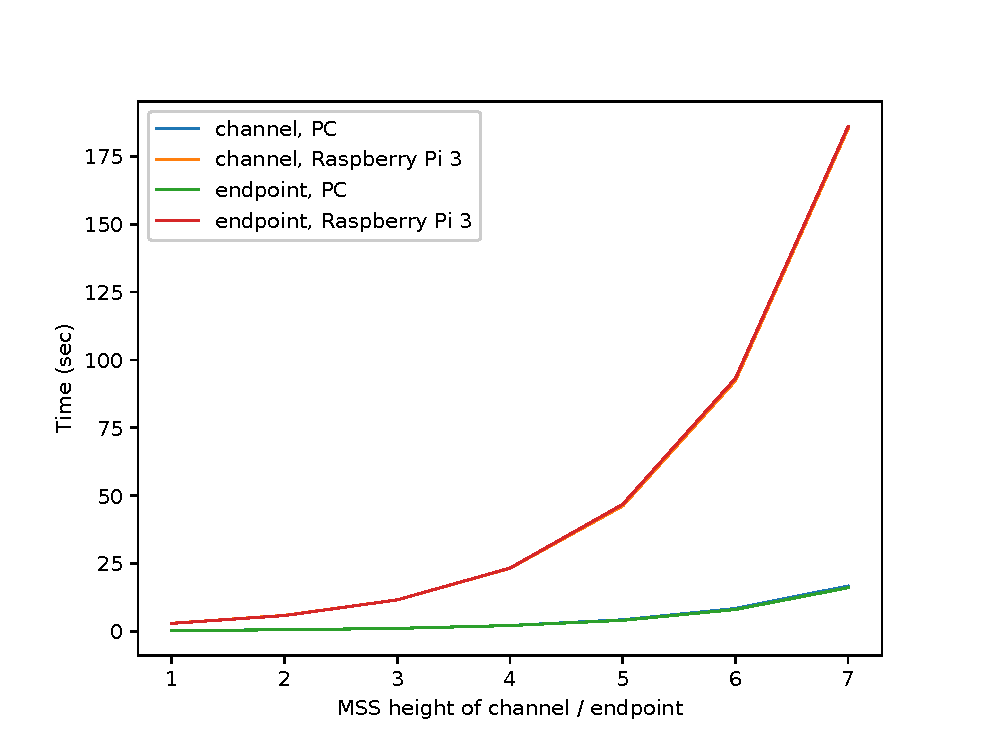
\includegraphics[width=2.5in]{mam_create}
    \caption{Time cost of MAM creation.}
    \label{fig:mam_create}
\end{figure}

\subsubsection{Messages Publishment}
Publishing a message to MAM is attaching a zero-value transaction to the Tangle which requires two processes:
\begin{itemize}
	\item	Tips selection: In the IOTA protocol, a new-coming transaction needs to pick up 2 existed transactions called tips to reference and verify. The tips are provided by IOTA full nodes.
	\item	Proof-of-Work (PoW): An algorithm which prevents Denial of Service and spam attacks on a network. A computationally hard puzzle to solve, but easy to verify. IOTA uses a Hashcash\cite{Hashcash} based puzzle.
\end{itemize}

Tips selection requires a stable network connection to wait the response from IOTA full nodes, and PoW requires enough computation resources to perform. Fig.~\ref{fig:mam_send} shows probability distribution function of publishing a message to MAM endpoint. The time of Raspberry Pi 3 distributed widely, since the randomness of PoW has huge impact while all the tests on PC remain in a possible range.

\begin{figure}[!t]
    \centering
    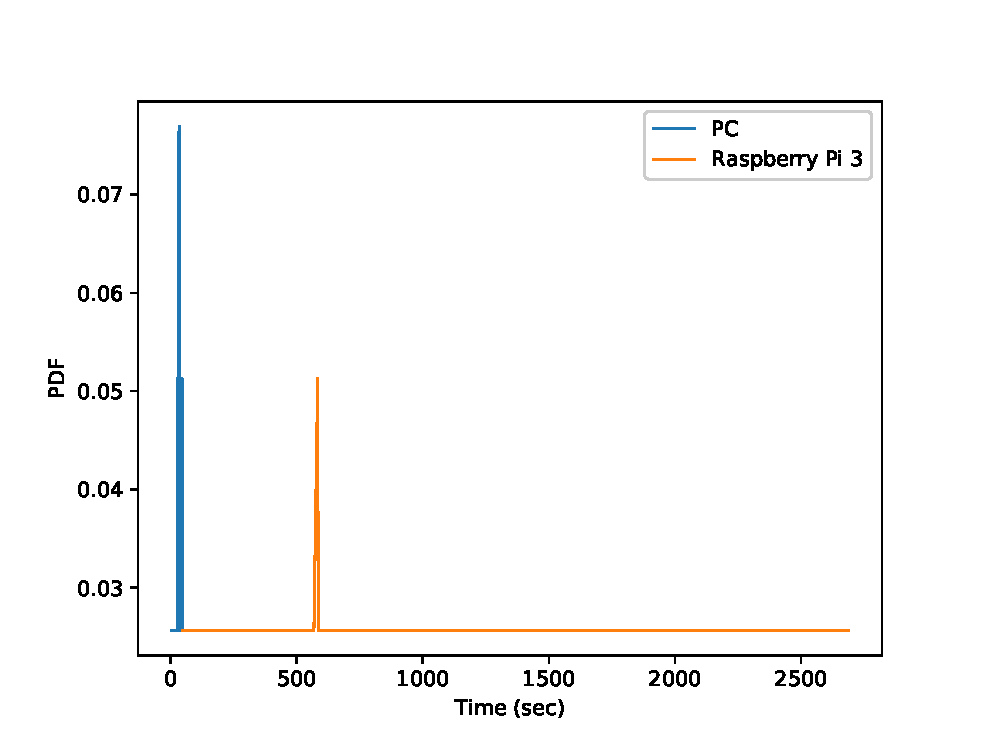
\includegraphics[width=2.5in]{mam_send}
    \caption{Time cost of sending a message through MAM.}
    \label{fig:mam_send}
\end{figure}

The simulation results above indicate that MAM is difficult for low-level sensor devices to run, whereas these kind of devices are the majority hardware in the IoT scenarios. Furthermore, sensors with the low computing power and unstable internet connection are not able to have enough resources to handle data collection, data transmission on MAM and even trading process with subscribers simultaneously. 

Therefore, transferring MAM operations to brokers while ensuring the profit and privacy of providers through blind signatures can effectively solve performance problems and lower the threshold to participate in such framework. Brokers can be PCs or powerful machines that runs Ethereum client and Tangle-accelerator\cite{TA}. Where Ethereum client is used to interact with Ethereum and Tangle-accelerator is a caching proxy server for IOTA, which can serve thousands of IOTA requests at once without accessing remote IOTA full nodes frequently and provide PoW acceleration. Fig.~ \ref{fig:ta_struct} shows the structure of Tangle-accelerator. However, MAM operations still cost a considerable time that improving the performance of MAM is an essential issue that needs to be done for the next step.  

\begin{figure}[!t]
    \centering
    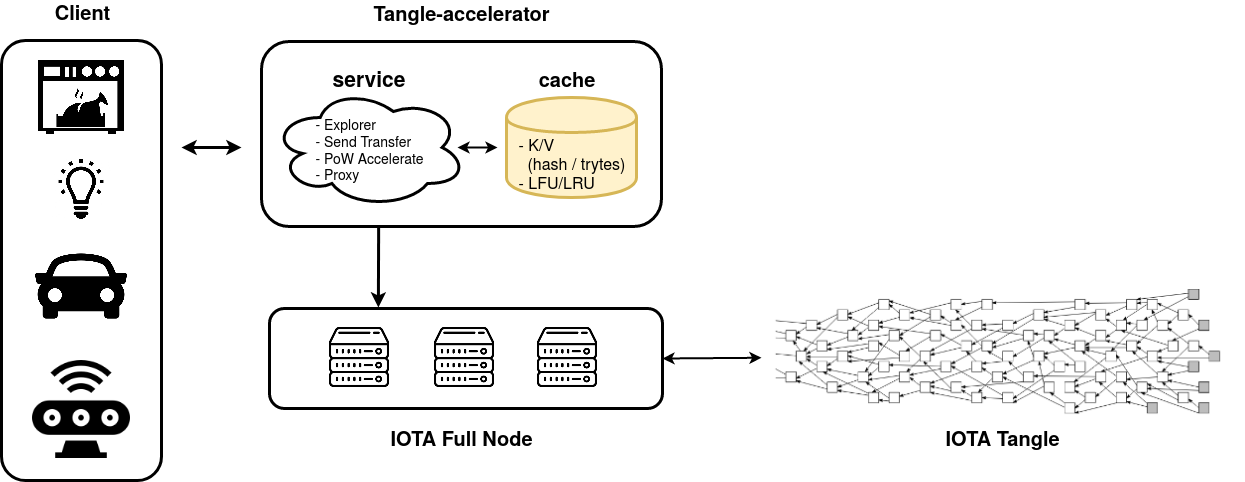
\includegraphics[width=3in]{ta_structure}
    \caption{The structure of Tangle-accelerator.}
    \label{fig:ta_struct}
\end{figure}

\section{Conclusions}
By combining the established standards and openly-developed specifications, this paper proposed an autonomous publish/subscribe model design to serve as a vendor and industry-neutral platform, automating the trading of digital assets and services. It was built with blockchain network, immutable audit trails, and contracts with an integrated decentralized identity system, to ensure the authenticity of all participants and enable secure communication and flexible trading mechanisms.

\bibliographystyle{IEEEtran}
\bibliography{references}

\end{document}
